\documentclass[14pt,pdf,hyperref={unicode}]{beamer}

% \documentclass[aspectratio=43]{beamer}
% \documentclass[aspectratio=1610]{beamer}
% \documentclass[aspectratio=169]{beamer}

\usepackage{lmodern}

% подключаем кириллицу 
\usepackage[T2A]{fontenc}
\usepackage[utf8]{inputenc}
\usepackage{listings}
\usepackage{graphicx}
\usepackage{hyperref}

% отключить клавиши навигации
\setbeamertemplate{navigation symbols}{}

% тема оформления
\usetheme{CambridgeUS}

% цветовая схема
\usecolortheme{seahorse}

\definecolor{light-gray}{gray}{0.90}

\lstset{basicstyle=\ttfamily,breaklines=true}

\title{Семинар №12}   
\subtitle{ФАКИ 2015}
\author{Бирюков В. А.} 
\date{\today} 
% \logo{\includegraphics[height=5mm]{images/logo.png}\vspace{-7pt}}

\begin{document}

\lstset{language=C}

% титульный слайд
\begin{frame}
\titlepage
\end{frame} 



\defverbatim[colored]\makeset{
\begin{lstlisting}[language=C++,basicstyle=\ttfamily,keywordstyle=\color{blue},
                stringstyle=\color{red}\ttfamily]
void make_set(int X) {
  parent[X] = X;
}
\end{lstlisting}
}

\lstset{
  language=C,                % choose the language of the code
  keywordstyle=\color{blue},
  numbers=none,                   % where to put the line-numbers
  stepnumber=1,                   % the step between two line-numbers.        
  numbersep=5pt,                  % how far the line-numbers are from the code
  backgroundcolor=\color{light-gray},  % choose the background color. You must add \usepackage{color}
  showspaces=false,               % show spaces adding particular underscores
  showstringspaces=false,         % underline spaces within strings
  showtabs=false,                 % show tabs within strings adding particular underscores
  tabsize=2,                      % sets default tabsize to 2 spaces
  captionpos=b,                   % sets the caption-position to bottom
  breaklines=true,                % sets automatic line breaking
  breakatwhitespace=true,         % sets if automatic breaks should only happen at whitespace
}








\section{Указатели}
\begin{frame}
\begin{center}
\begin{beamercolorbox}[sep=8pt,center]{part
title}
\usebeamerfont{part title}\insertsection
\end{beamercolorbox}
\end{center}
\end{frame}


\begin{frame}[fragile]
\frametitle{Указатели} 
\framesubtitle{Адрес переменной}
\begin{center}
\includegraphics[width=0.95\linewidth]{images/memory_pointer_2.png}
\end{center}
\end{frame}


\begin{frame}[fragile]
\frametitle{Указатели} 
\framesubtitle{Ссылка по указателю}
\begin{center}
\includegraphics[width=0.95\linewidth]{images/memory_pointer_4.png}
\end{center}
\end{frame}


\begin{frame}[fragile]
\frametitle{Указатели и аргументы функций} 
\framesubtitle{Передача по значению}
\begin{center}
\includegraphics[height=0.55\linewidth]{images/swap_wrong.png}
\end{center}
\end{frame}

\begin{frame}[fragile]
\frametitle{Указатели и аргументы функций} 
\framesubtitle{Передача по адресу}
\begin{center}
\includegraphics[height=0.55\linewidth]{images/swap_right.png}
\end{center}
\end{frame}



\begin{frame}[fragile]
\frametitle{Указатели и массивы} 
\framesubtitle{Связь массивов и указателей}
\begin{center}
\includegraphics[width=0.95\linewidth]{images/memory_parrays_4.png}
\end{center}
\end{frame}






\section{Malloc и free. Управление памятью.}
\begin{frame}
\begin{center}
\begin{beamercolorbox}[sep=8pt,center]{part
title}
\usebeamerfont{part title}\insertsection
\end{beamercolorbox}
\end{center}
\end{frame}

\begin{frame}[fragile]
\frametitle{Управление памятью} 
\framesubtitle{Сегменты памяти процесса}
\begin{center}
\includegraphics[width=0.8\linewidth]{images/process_memory_organization.png}
\end{center}
\end{frame}

\begin{frame}[fragile]
\frametitle{Стек (Stack)} 
\begin{itemize}
\item Стек представляет собой обычный алгоритмический стек, применённый для управления памяти
\item В нём хранятся локальные переменные
\item Имеет фиксированный размер, определяется операционной системой, на порядок меньше чем Куча
\item Немного быстрее, чем Куча
\end{itemize}
\end{frame}

\begin{frame}[fragile]
\frametitle{Куча (Heap)} 
\begin{itemize}
\item Куча представляет собой обычную алгоритмическую кучу, применённую для управления памяти
\item В ней можно динамически выделять память
\item Размер, обычно, ограничен только доступными ресурсами
\item Немного медленней, чем Стек
\end{itemize}
\end{frame}


\begin{frame}[fragile]
\frametitle{Выделение памяти в Куче с помощью malloc и free} 
\framesubtitle{Выделение памяти на массив из 100 переменных типа int} 
\begin{center}
\includegraphics[width=0.55\linewidth]{images/malloc_free_2.png}
\end{center}
\end{frame}







\section{Структуры}
\begin{frame}
\begin{center}
\begin{beamercolorbox}[sep=8pt,center]{part
title}
\usebeamerfont{part title}\insertsection
\end{beamercolorbox}
\end{center}
\end{frame}



\begin{frame}[fragile]
\frametitle{Структуры} 
\framesubtitle{Пример} 
Описание структуры:
\begin{lstlisting}[language=C++,basicstyle=\ttfamily,keywordstyle=\color{blue}]
struct account {
   int account_number;
   char first_name[30];
   char last_name[50];
   float balance;
};
\end{lstlisting}
Объявление структуры:
\begin{lstlisting}[language=C++,basicstyle=\ttfamily,keywordstyle=\color{blue}]
struct account ac1;
\end{lstlisting}
\end{frame}



%E9C6AF
%C6E9AF


\section{Стек и очередь}
\begin{frame}
\begin{center}
\begin{beamercolorbox}[sep=8pt,center]{part
title}
\usebeamerfont{part title}\insertsection
\end{beamercolorbox}
\end{center}
\end{frame}



\begin{frame}[fragile]
\frametitle{Стек} 
\begin{center}
\includegraphics[width=0.8\linewidth]{images/Lifo_stack.png}
\end{center}
\end{frame}


\begin{frame}[fragile]
\frametitle{Стек} 
\framesubtitle{Описание стека} 

\begin{lstlisting}[language=C++,basicstyle=\ttfamily,keywordstyle=\color{blue}]
#define N 100
typedef int Data;

struct Stack {
    int n;
    Data a[N];
};
\end{lstlisting}
\end{frame}


\begin{frame}[fragile]
\frametitle{Очередь} 
\begin{center}
\includegraphics[width=0.8\linewidth]{images/queue.png}
\end{center}
\end{frame}




\section{Быстрая сортировка}
\begin{frame}
\begin{center}
\begin{beamercolorbox}[sep=8pt,center]{part
title}
\usebeamerfont{part title}\insertsection
\end{beamercolorbox}
\end{center}
\end{frame}

\begin{frame}[fragile]
\frametitle{Быстрая cортировка (quicksort)} 
\begin{center}
\includegraphics[width=0.9\linewidth]{images/qs1.png}
\end{center}
\end{frame}

\begin{frame}[fragile]
\frametitle{Быстрая cортировка (quicksort)} 
\begin{center}
\includegraphics[width=0.9\linewidth]{images/qs2.png}
\end{center}
\end{frame}


\begin{frame}[fragile]
\frametitle{Время работы сортировок} 
\begin{itemize}
\item Время работы сортировки пузырьком, выбором и вставками $\sim n^2$ \\
\item Время работы сортировки слиянием и быстрой сортировки в среднем $\sim n log(n)$ \\
\end{itemize}
\end{frame}



\begin{frame}[fragile]
\frametitle{Стандартная сортировка qsort()} 
\begin{lstlisting}[language=C++,basicstyle=\ttfamily,keywordstyle=\color{blue}]
#include <stdlib.h>
int values[] = { 88, 56, 100, 2, 25 };

int cmp(const void * a, const void * b)
{
   return ( *(int*)a - *(int*)b );
}
...
qsort(values, 5, sizeof(int), cmp);

\end{lstlisting}
\end{frame}












\section{Функция main}
\begin{frame}
\begin{center}
\begin{beamercolorbox}[sep=8pt,center]{part
title}
\usebeamerfont{part title}\insertsection
\end{beamercolorbox}
\end{center}
\end{frame}


\begin{frame}[fragile]
\frametitle{Функция main}  
\begin{center}
\includegraphics[width=0.7\linewidth]{images/function_syntax_main_args.png}
\end{center}
\begin{itemize}
\item argv -- параметры, передаваемые в функцию main
\item argc -- количество этих параметров
\end{itemize}
\end{frame}

\begin{frame}[fragile]
\frametitle{Функции} 
\framesubtitle{Функция main}
\begin{center}
\includegraphics[width=1.0\linewidth]{images/function_argcargv.png}
\end{center}
\end{frame}




\section{Запись/чтение файлов}
\begin{frame}
\begin{center}
\begin{beamercolorbox}[sep=8pt,center]{part
title}
\usebeamerfont{part title}\insertsection
\end{beamercolorbox}
\end{center}
\end{frame}


\begin{frame}[fragile]
\frametitle{fprintf, fscanf}  
\begin{lstlisting}[language=C++,basicstyle=\ttfamily,keywordstyle=\color{blue},
                stringstyle=\color{orange}\ttfamily]
   #include <stdio.h>
   FILE *fptr;
   fptr=fopen("output.txt", "w");
   if(fptr==NULL){
      printf("Error!");   
      exit(1);             
   }
   fprintf(fptr, "%d", n);   
   fclose(fptr);
\end{lstlisting}
\end{frame}


\begin{frame}[fragile]
\frametitle{fputc, fgetc}  
\begin{lstlisting}[language=C++,basicstyle=\ttfamily,keywordstyle=\color{blue},stringstyle=\color{orange}\ttfamily]
   FILE * f = fopen("input.txt", "r");
   
   int number_of_chars = 0;
   int c;
   
   while ((c = fgetc(f)) != EOF)
   {
       number_of_chars++
   }
   fclose(f);
\end{lstlisting}
\end{frame}

\begin{frame}[fragile]
\frametitle{Бинарные чтение/запись}  
\framesubtitle{fread, fwrite}  
\begin{lstlisting}[language=C++,basicstyle=\ttfamily,keywordstyle=\color{blue},stringstyle=\color{orange}\ttfamily]
   char c[] = "some string data";
   char buffer[100];
   FILE *fp = fopen("output.txt", "w+");
   fwrite(c, strlen(c) + 1, 1, fp);
   fclose(fp);
\end{lstlisting}
\end{frame}








\section{Структуры данных}
\begin{frame}
\begin{center}
\begin{beamercolorbox}[sep=8pt,center]{part
title}
\usebeamerfont{part title}\insertsection
\end{beamercolorbox}
\end{center}
\end{frame}




\begin{frame}[fragile]
\frametitle{Структуры данных}
\begin{itemize}
\item Структура данных (англ. data structure) — определённый способ организации данных, так, чтобы их можно было использовать эффективно.
\item Для разных задач более эффективными будут разные структуры данных.
\end{itemize}
\end{frame}


\begin{frame}[fragile]
\frametitle{Упорядоченный массив}
\begin{center}
  \begin{tabular}{  l | c r }
      & Массив & Упорядоченный массив \\
    \hline
    index & O(1) & O(1)\\
    insert & O(1) & O(N)\\
    remove & O(N) & O(N)\\
    find & O(N) & O($\log(N)$)\\
    \hline
  \end{tabular}
\end{center}
\end{frame}



\begin{frame}[fragile]
\frametitle{Связный список} 
\begin{lstlisting}[language=C++,basicstyle=\ttfamily,keywordstyle=\color{blue},stringstyle=\color{orange}\ttfamily]
struct Node {
	int data;
	struct Node * next;
};
struct Node * head;
\end{lstlisting}
\end{frame}



\begin{frame}[fragile]
\frametitle{Связный список} 
\framesubtitle{Обход связного списка - 1} 
\begin{center}
\includegraphics[width=0.99\linewidth]{images/list_traversal_1.png}
\end{center}
\end{frame}
\begin{frame}[fragile]
\frametitle{Связный список} 
\framesubtitle{Обход связного списка - 2} 
\begin{center}
\includegraphics[width=0.99\linewidth]{images/list_traversal_2.png}
\end{center}
\end{frame}
\begin{frame}[fragile]
\frametitle{Связный список} 
\framesubtitle{Обход связного списка - 3} 
\begin{center}
\includegraphics[width=0.99\linewidth]{images/list_traversal_3.png}
\end{center}
\end{frame}




\begin{frame}[fragile]
\frametitle{Двусвязный список}
\begin{center}
  \begin{tabular}{  l | c r }
      & Список & Двусвязный список \\
    \hline
    index & O(N) &  O(N) \\
    insertToFront & O(1) & O(1) \\
    insertToBack & O(N) & O(1) \\
    insertAfter & O(1) & O(1) \\
    insertBefore & O(N) & O(1) \\
    remove & O(1) & O(1) \\
    find & O(N) & O(N) \\
    \hline
  \end{tabular}
\end{center}
\end{frame}







\section{Задание}
\begin{frame}
\begin{center}
\begin{beamercolorbox}[sep=8pt,center]{part
title}
\usebeamerfont{part title}\insertsection
\end{beamercolorbox}
\end{center}
\end{frame}

\begin{frame}[fragile]
\frametitle{Задание} 
\begin{itemize}
\item Тренировочная к/р №2
\end{itemize}
\end{frame}

\end{document}
